\chapter{Implementation}
This chapter will be a thorough explanation of the implementation of the prototype.
As described in the design chapter the following is what will be implemented:
\begin{itemize}
\item 3D level
\item 3 control schemes:
		\begin{itemize}
		\item Joystick Controller
		\item Buttons Controller
		\item Gyroscopic Controller 
		\end{itemize}
\item A script that will enable all the controllers to work with buttons.
\end{itemize}

\section{Unity Introduction}
For this implementation the choice was made to use the freely available Unity3D engine. This was chosen as Unity provides a lot of features that would otherwise mean that this project would not be possible to complete in the amount of time given. This section will provide a quick glance at what Unity is and introduce some common terms used within Unity. Everything that is seen in a Unity game is composed of {\tt GameObjects}. These objects are what the scripts described in the following sections will be attached to. A newly created {\tt GameObject} will only contain what is known as a {\tt Transform}. The transform is an object that holds the information about where the object is within the 3D space. It also holds the objects rotational information  and its scale.
The position of the object is expressed as a vector. A vector is a mathematical tool for representing a coordinate in space. As such, vectors are the primary tool that is used in unity for expressing things like velocity, position, forces etc.
\section{Development of 3D elements}
The actual implementation consisted of creating level areas, 3D prefabs; cones, poles with string, sprites, notes and arrows. 3D elements were created using the software "Maya", which is a 3D modelling and animation programme. Textures were made with "Photoshop". Each level started by a simple creation of a square representing a room. Then considerations of what the test should include were done and assets were placed to make different challenges. Picture \ref{3dDevelopment1} shows a 3D cone and its texture.
\begin{figure}[H]
\centering
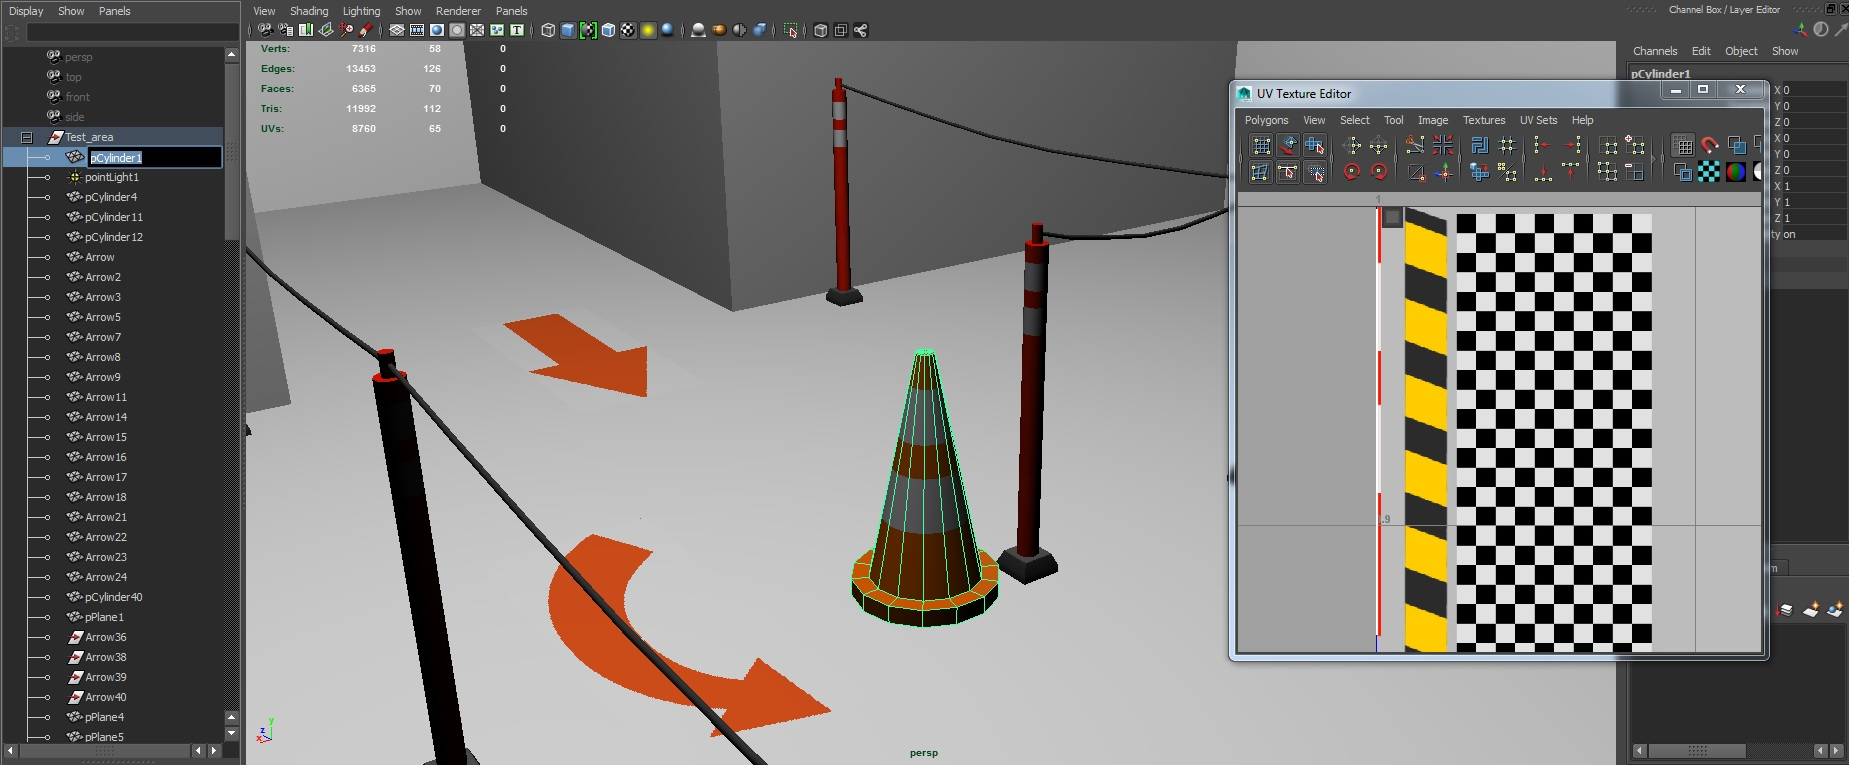
\includegraphics[scale=0.35]{3D_dev_7.jpg}
\caption{Picture of a cone from the testing level}
\label {3dDevelopment1}
\end{figure}
Every object that required texturing, also needed its own UV map. UV maps are a three dimensional model representation in two dimensions. This helps to see where to paint textures using tools as Photoshop. Following picture \ref{3dDevelopment2} shows UV map as red lines, that helps to see the boundaries for the texturing in Photoshop.
\begin{figure}[H]
\centering
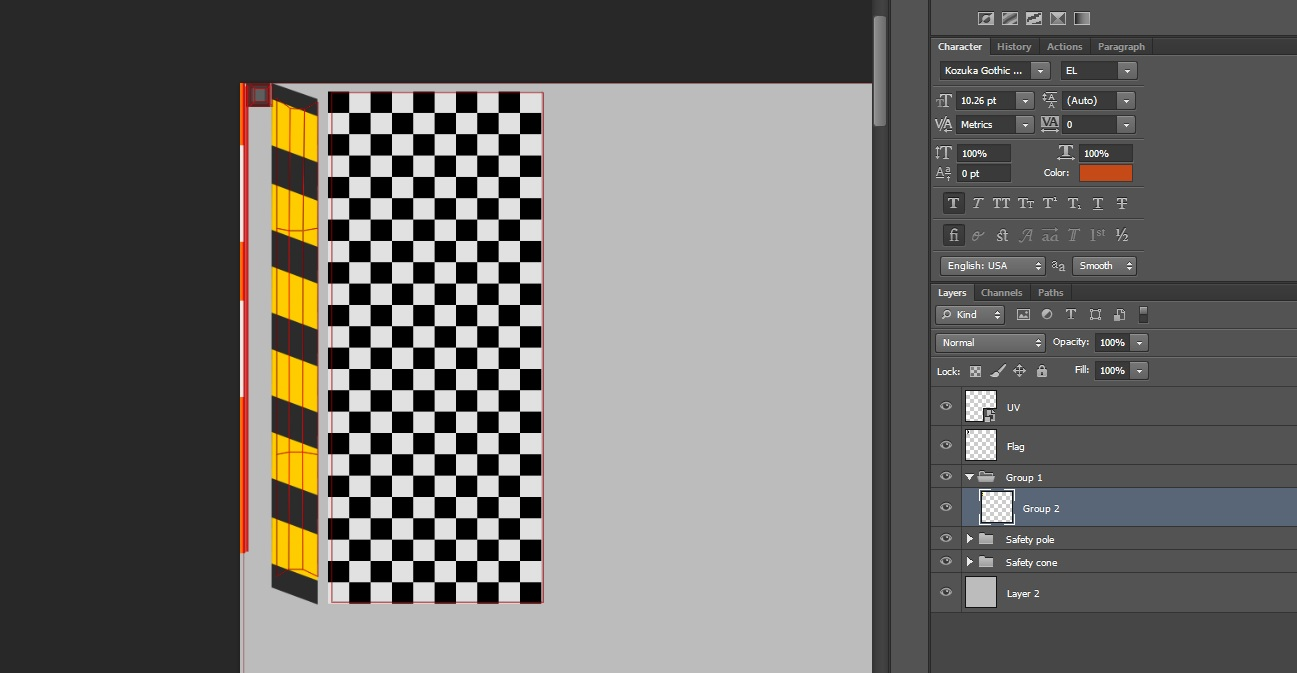
\includegraphics[scale=0.35]{3D_dev_8.jpg}
\caption{Picture of a cone from testing level}
\label {3dDevelopment2}
\end{figure}
Text, directional arrows and other symbols needed to be transparent so it would blend well with most of the background, see fig. \ref {3dDevelopment3}. Such images were exported as .png picture format to reserve the transparency. 

\begin{figure}[H]
\centering

\includegraphics[scale=0.3]{3D_dev_9.png}
\caption{Pictures of elements that required transparency for game engine, also called sprites.}
\label{3dDevelopment3}
\end{figure}

Since graphics and aesthetics were not the focus of this test level, textures were created very minimalistic without any shadowing, noise, imitation of being old/used etc. It also helped making the test optimized for hardware performance, since the textures size on a disk were as little as a few kilobytes.

\section{Buttons}
The buttons used in all three schemes are all created using unity's UI system. A button in the UI system is just an empty {\tt GameObject} that holds the following components:
\begin{itemize}
\item {\tt Rect Transform}\\
This component is equivalent to the regular {\tt Transform}. This component does not contain any information about the objects position in 3D space though, as it is part of the UI it only needs to know its coordinates on a 2D plane. The UI system provides a convenient way of making sure that the UI will look the same, no matter what screen size is used. It does this by having coordinates relative to an anchor point that is set by the developer. 
\item {\tt Button}\\
This is the standard script that unity uses to detect clicks on a button and can call methods on different objects when clicked. This script is the script that has been modified to allow for pressing and holding.
\item {\tt Image} \\
This component is a component that will draw an image on the canvas. This image will be the full size of the button.
\end{itemize}

\subsection{{\tt ButtonScript}}
{\tt ButtonScript} inherits from the in-built Unity {\tt Button} object. This is done so that the script can access the method {\tt   protected bool IsPressed()}. This script is the one that all buttons in both the buttons and gyroscope scene uses. It is a simple extension. All it has to do is to check if the button is being pressed and if it is, then check which button it is and act accordingly. 
\section{Buttons Scene}
The button scene is the only scene that only uses  {\tt CamMovement} and {\tt ButtonScript} and is therefore the simplest scene technically. Presented below is  the methods contained within {\tt camMovement}: 
\begin{itemize}
\item {\tt public void move(bool rightButton)}\\
This method will, depending on the boolean given to it, move the camera forward or backward. This is done by creating a directional vector formed from the transforms forward vector:
\begin{verbatim}
Vector3 directionVector = new Vector3(transform.forward.x, 
                                      0,
                                      transform.forward.z)
\end{verbatim}
The directional vector will always have a y component of 0 as the camera should not be able to move in the y direction. This vector is then multiplied by an integer variable that will take the value of either -1 or 1, depending on the value of {\tt rightButton} by converting the boolean into an integer with the line:\\
{\tt int goingForward = rightButton ? -1 : 1;}\\
Finally the directional vector is multiplied with a variable for determining the speed of the movement. This directional vector is then set as the velocity of the rigid body that is attached to the GameObject. 

\item {\tt public void rotateLeftRight(bool right)}\\
This method will rotate the camera left or right in a similar manner to {\tt move}. But where {\tt move} does not do anything to its y component, the {\tt rotateLeftRight} method will only rotate in its y component and keep the rotation of the x component. This method uses {Quaternion.euler } to convert our euler angles into Quaternions and {\tt Quaternion.Slerp} to smoothly make the camera rotate. This can be seen in figure \ref{Slerping}.
 
\begin{figure}[H]
\centering
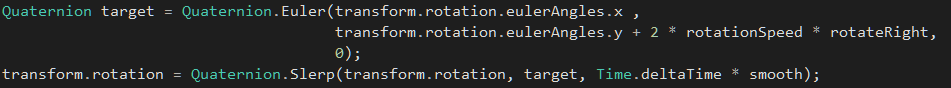
\includegraphics[scale=0.8]{Slerping.PNG}
\caption{Conversion of quaternions into euler angles and use of the slerp function.}
\label{Slerping}
\end{figure}

\item {\tt public void rotateUpDown(bool down)}\\
This function is more or less the exact same as {\tt rotateLeftRight} but where {\tt rotateLeftRight} makes changes to the y component of the rotation, {\tt rotateUpDown} rotates the x component. 

\item {\tt public void stopMovement()}\\
This function is a simple function to make all movement on the camera stop. It will set both the linear and angular velocity of the object to zero.
\end{itemize}

\section{Gyroscope Camera}
The gyroscopic camera uses two scripts to work, first and most importantly the {\tt GyroController} which is the script responsible for getting the input from the gyroscope and rotating accordingly. Unity can take inputs from the gyroscope directly but if an object is rotated by the raw data from the gyroscope, there will immediately be a problem as the coordinate system that is used by the gyroscope is a right-handed coordinate system
 
\begin{figure}[H]
\centering
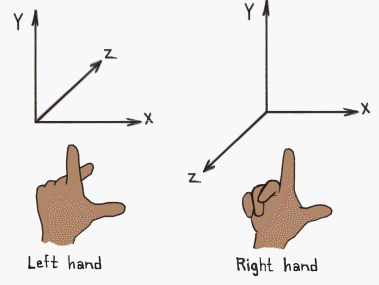
\includegraphics[scale=0.8]{left_right_hand.png}
\caption{Right-handed vs. left-handed coordinate systems}
\end{figure}

where unity uses a left hand coordinate system. To have the coordinates given by the gyroscope match the coordinates of Unity, the {\tt GyroController} has a method for converting from right-handed to left-handed coordinate systems. This method uses Quaternions which is how Unity handles rotation internally, explaining quaternions is beyond the scope of this project.\label{quaternions}
Besides the {\tt GyroController}, this scene also uses the {\tt CamMovement} and {\tt ButtonScript} explained in the previous section. In this scene, only the forward and backward buttons are used though, as the gyroscope is handling the rotation of the camera.
\section{Joystick Scene} 
The joystick scene is technically the most difficult it uses some of Unity's standard assets, these include:

\subsection*{Mobile Joystick}
The mobile joystick script creates two axis for unity's input manager. These two axis are then accessed by the first person controller and uses these values to move the camera. 
\subsection*{The Character controller}
This is actually a fully fleshed component along with components like the transform, renderer etc. For this scene it is primarily used to generate a collider for the camera. 
\subsection*{First Person Controller}
Unity provides a standard first person controller that comes with a whole range of features. For this scene the first person controller needs to take inputs from the joystick. To do this the first person controller's {\tt RotateView()} method has been modified to take input from the virtual axis created by the mobile joystick:

\begin{figure}[H]
\centering
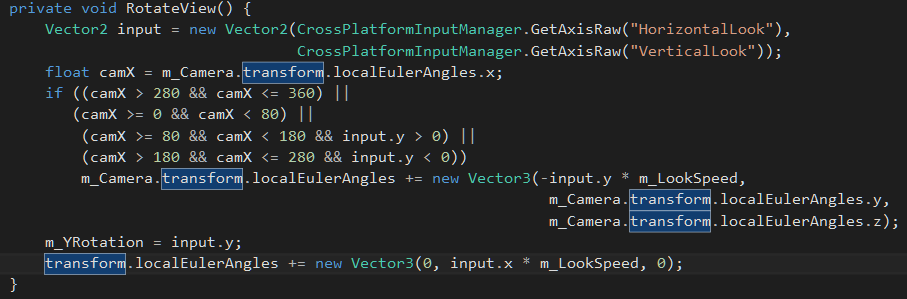
\includegraphics[scale=0.9]{RotateViewFunction.PNG}
\caption{The modified {\tt RotateView()} from the first person controller.}
\end{figure}

This method reads the input from the axis named {\tt HorizontalLook} and {\tt VerticalLook} and stores these two values in a vector. This vector is essentially the directional vector we want to add to the camera's rotation. While a solution such as;
\begin{verbatim}
Vector3 dVector = new Vector3(input.x,input.y,0);
transform.localEulerAngles += dVector;
\end{verbatim} will make the transform rotate in the direction of the vector, it will also cause the camera angles to get stuck. This problem is known as gimbal locking, which is the situation where two rotational axis is pointing in the same direction. To avoid this problem the script checks to make sure that the camera is not rotated into a gimbal lock and adds the rotation to the local rotation of the camera. The script does this by checking if the user is looking down or up at an angle of less than 80 degrees. 